\section{Comparison Matrices}\label{sec:matrix}

% ANTOINE -> TODO

% TODO - From reviewer 1 : Section 4.1: The section present a way to select papers, but it is not clear how to select papers concretely. The last three paragraphs in Section 4.1 should be expanded.

In this paper, we propose three matrices to assist the architect in his task of selecting the right technologies to build a Semantic REST system. As we showed in the previous section, the WS3 classification is too coarse-grained to grasp all important differences between systems of the same maturity level. Therefore, presented matrices compare the technologies along a set of precise criteria to highlight these differences.

In this section we present the methodology that we followed to select the technologies and classification criteria, we present the matrices and leverage them to draw a high-level comparison of the technologies. Criteria are categorized by the levels of WS3 or within a "other" category with criteria that cannot be linked to one level of WS3 but are useful to highlight differences between technologies.

Among available technologies, we distinguished three categories: (i) Interface Description Languages (IDL); (ii) data-interchange formats, which provide a data-structure, a vocabulary and a layout to represent a resource and its meta-data and (iii) implementation frameworks. One matrix is presented per category.

\subsection{Comparison Matrices Design Methodology}

% TODO - IN PROGRESS - From reviewer 2 : My impression is that the paper only accounts the result of the web search, and developers' expertise is not actually leveraged. Which are the daily problems developers face? Go deeper with their experience. The framework is intended to be used by developers, you should take into account their insights from the trenches. Interview people from your company if needed, and provide links to their responses/questionnaires.

% TODO - From reviewer 2 : The methodology steps can be shortened, as they do not add any useful information. How did you verified the criteria (step v) w.r.t. your previous projects? Provide an example.

The design of the comparison matrix follows a 5 steps sequential process: (i) looking for candidate technologies, (ii) selecting candidate technologies, (iii) deep reading and understanding of each candidate technology, (iv) elaboration of fine grain criteria to characterize and differentiate technologies, (v) double-verification that the elaborated criteria highlighted the differences between technologies.
% maybe merge (v) and (vi)

The research of candidate technologies (step i) was done by:

\begin{enumerate}
    \item Searching Google and Google Scholar for Semantic REST Technologies using compositions of keywords from the set: ["web", "semantic", "restful", "rest", "service", "API", "interface", "description", "documentation", "language", "modeling", "hypermedia", "document", "format", "RDF", "data-interchange", "media-type", "linked data", "hateoas", "rest api", "framework"]
    \item Searching Google Scholar for tools automating tasks from services description, using keywords: "matchmakers", "service composition", "service discovery", "rest service analysis", "automated mashups". We then selected other papers and technologies from their references and the papers that cite the ones we selected.
    \item Looking at papers related to documenting, implementing and evaluating Web APIs from the proceedings of ICWE and WS-REST. 
\end{enumerate}

% Maybe update the 81 number below if the Github with raw material changes.
From these researches, we selected 81 papers (step ii), standards, articles and web pages from their abstract or introduction. To be selected, documents had to be the specification of an interface definition language or model, a framework that supports HATEOAS features, an interchange format that supports RDF or HATEOAS features, a comparison between these technologies or a tool leveraging them. Frameworks to build Semantic Web Services were excluded because they are based on triples which are too far from the resource-centric approach of REST. We opened our research to technologies from the 1990s to today and retained technologies that are still available today.

As a next step, we read the specification of each chosen technology (step iii) and elaborate classification criteria (step iv). Some criteria targeting interchange formats are the H Factor\footnote{\url{http://amundsen.com/hypermedia/hfactor/}}. Others were carefully designed to highlight differences between technologies in the area of Semantic REST, based on the core design of the technologies, the features they provide and the details of the WS3 maturity model. Several steps of refinement were needed to avoid duplicating criteria or hiding details. All the raw material used to elaborate this classification is available online\footnote{\url{https://github.com/AntoineCheron/semantic-restful-api-technologies-comparison-matrix}}. 
% TODO @Johann @Olivier: the above paragraph needs to be reviewed. If not good enough, I will need help to improve it.

As a final step (step v), we read the specifications again to validate that the selected criteria highlighted differences and commonalities well, and to verify results.

\paragraph{Popularity criteria}

% Long version
%We included a popularity criteria to offer a vague idea of whether a community might help with any problem that may arise and how likely the technology will be lasting. The popularity score is between 0 and 2. The highest, the more popular the technology is. To score technologies we took several indicators into account. First, the number of questions about the technology on Stack Overflow\footnote{\url{https://stackoverflow.com}}. Then, for IDL and interchange formats only, we looked at the five most popular libraries on NPM\footnote{\url{https://www.npmjs.com/}} and Maven Central\footnote{\url{https://mvnrepository.com/repos/central}}. On NPM we selected the weekly downloads and on Maven, the usages. On the other hand, for the frameworks we collected the total downloads from the main repository of its language. The popularity score is computed as follows:

%Short version
We included a popularity criteria to offer a vague idea of whether a community might help with any problem that may arise and how likely the technology will be lasting. The popularity score is between 0 and 2. The highest, the more popular the technology is. The popularity score is computed as follows:

\begin{itemize}
    \item 0 - Not enough to reach 1
    \item 1 - More than 100 questions on stack overflow AND (2500+ NPM weekly downloads OR 100+ maven usages)
    \item 2 - More than 400 questions on stack overflow AND (more than 500.000 total downloads OR more than 15.000 NPM weekly downloads OR more than 500 maven usages)
\end{itemize}

% Antoine : continue from here
\subsection{Interface Description Languages}

Interface Description Languages (IDLs) provide a vocabulary to document domain, functional and non-functional aspects of an API. Non-RDF IDLs are tied to a fixed set of file formats. We also consider meta-models describing Web APIs, which are IDLs not tied to a file format, in this section. We identified 16 candidates that are classified according to 31 criteria in Fig~\ref{idl-matrix}.

When IDLs and data-interchange formats are both compatible with RDF, they can be combined to form a file format that can be used as both the data-interchange format and the IDL. This has great benefits in terms of complexity and maintainability.

\paragraph{Meta-Models}

Among the classified IDLs, 4 are meta-models. In \cite{Rapido} authors present a tool to sketch CRUD or Hypermedia APIs. When selecting Hypermedia APIs, the user skteches the application using state machines and obtain a result in the HAL or Collection+JSON format. \cite{Schreier:2011:MRA:1967428.1967434} models each resource type as a finite state machine with deterministic state transitions. In this model, each resource type has a single initial state, operations can go beyond CRUD and conditions can be modeled to inform the availability of operations. However, conditions are not modeled in more details, which does not make them machine-interpretable. In \cite{10.1007/978-3-642-22233-7_24}, authors propose to model the whole system as a non-deterministic state machine. This method makes software agents unable to discover the set of messages to exchange in order to make an operation available. Haupt et al. \cite{10.1109/ICWS.2014.30} propose a thorough multi-layered model that separates the domain model from the URI model. It does not allow specifying conditions on the availability of operations and see resources as having a static structure, making it impossible to represent different state of a resource with different classes. 

\subsubsection{Meta-Models from Interface Description Languages}

The 11 interface description languages we found are Hydra Core Vocabulary \cite{Lanthaler:2013:CGW:2487788.2487799}, Atom Syndication Format\cite{AtomSF}, WSDL+SAWSDL, WADL, OpenApi (used by Swagger), API Blueprint, hREST + microWSMO, RESTdesc, RADL, RAML and I/O Docs. We decided to include WSDL+SAWSDL even though it targets web services \cite{john2012framework} because it tackles the problem of semantically describing HTTP services.

% FIGURE OF THE IDL CLASSIFICATION
\begin{figure*}[Ht]
\caption{Interface Description Languages Comparison Matrix}
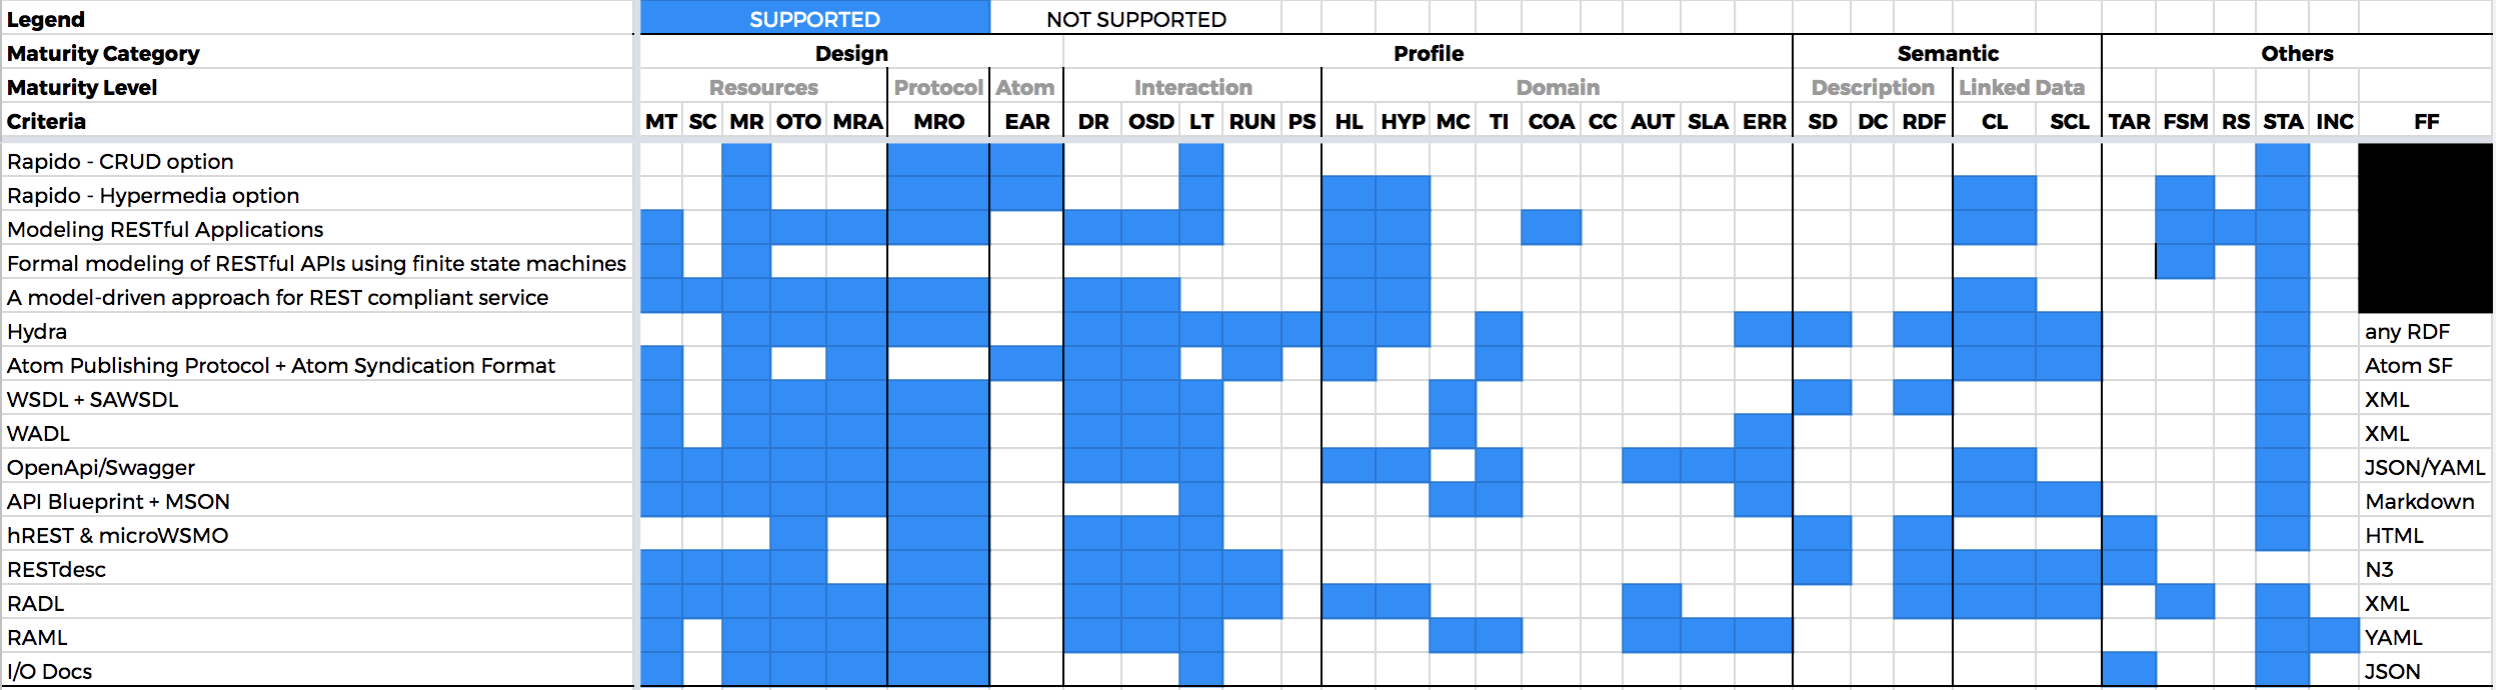
\includegraphics[width=1\textwidth]{figures/IDL.png}
\label{idl-matrix}
\end{figure*}

\subsubsection{Conclusions}

The first thing the matrix highlights is that most IDLs ignore the domain and semantic description of APIs. In addition, they focus on the static documentation of the entire API made for developers, rather than the documentation enriched with information on the current state of the system to guide users when browsing the API.

From this matrix, we observe that Hydra and RESTdesc are the two approaches reaching the highest maturity level. This is because they both semantically describe meta-data, use additional RDF vocabularies and target API documentation enriched with execution information.

Only one approach \cite{Schreier:2011:MRA:1967428.1967434} support conditional availability of links between resources and no one makes this meta-data machine-interpretable. This makes software agents unable to find a way to make an operation available when it is not.

Four technologies support the addition of business constraints to the model, and three are machine-processable. We encourage authors of meta-models to add this feature to their technology because it lowers coupling and improves user experience. For example, this allows forms to be automatically generated with client-side data validation.

Finally, this matrix highlights that three out of four scientific publications recommend the modeling of RESTful systems as state machines whereas all except one IDL authors ignore this technique. However, the use of deterministic state machines encourages API designers to think about the domain model in depth. It is then easier to determine if an operation on a resource is not available.

\subsection{Data-interchange formats}

The data-interchange formats can be differentiated based on their compatibility with RDF, which determines if they are extensible. Because they are extensible, RDF formats propose very few features by default. We selected three vocabularies (i) Hydra, (ii) HTTP RDF and (iii) SHACL, an RDF schema validation vocabulary, that we combined with one RDF format, JSON-LD, to show what is possible to do.

When building an API that provides no meta-data, JSON, XML and YAML are the three formats the most widely used in industry.

On the other side, when the system to build have to send meta-data, no interchange format is considered as a standard today. We found eleven candidates from our research. They are classified in Fig. \ref{interchange-formats-matrix} according to 26 criteria. % TODO : update the number of criteria

% FIGURE OF THE INTERCHANGE FORMATS CLASSIFICATION
\begin{figure*}[Ht]
\caption{Data-interchange Formats Comparison Matrix}
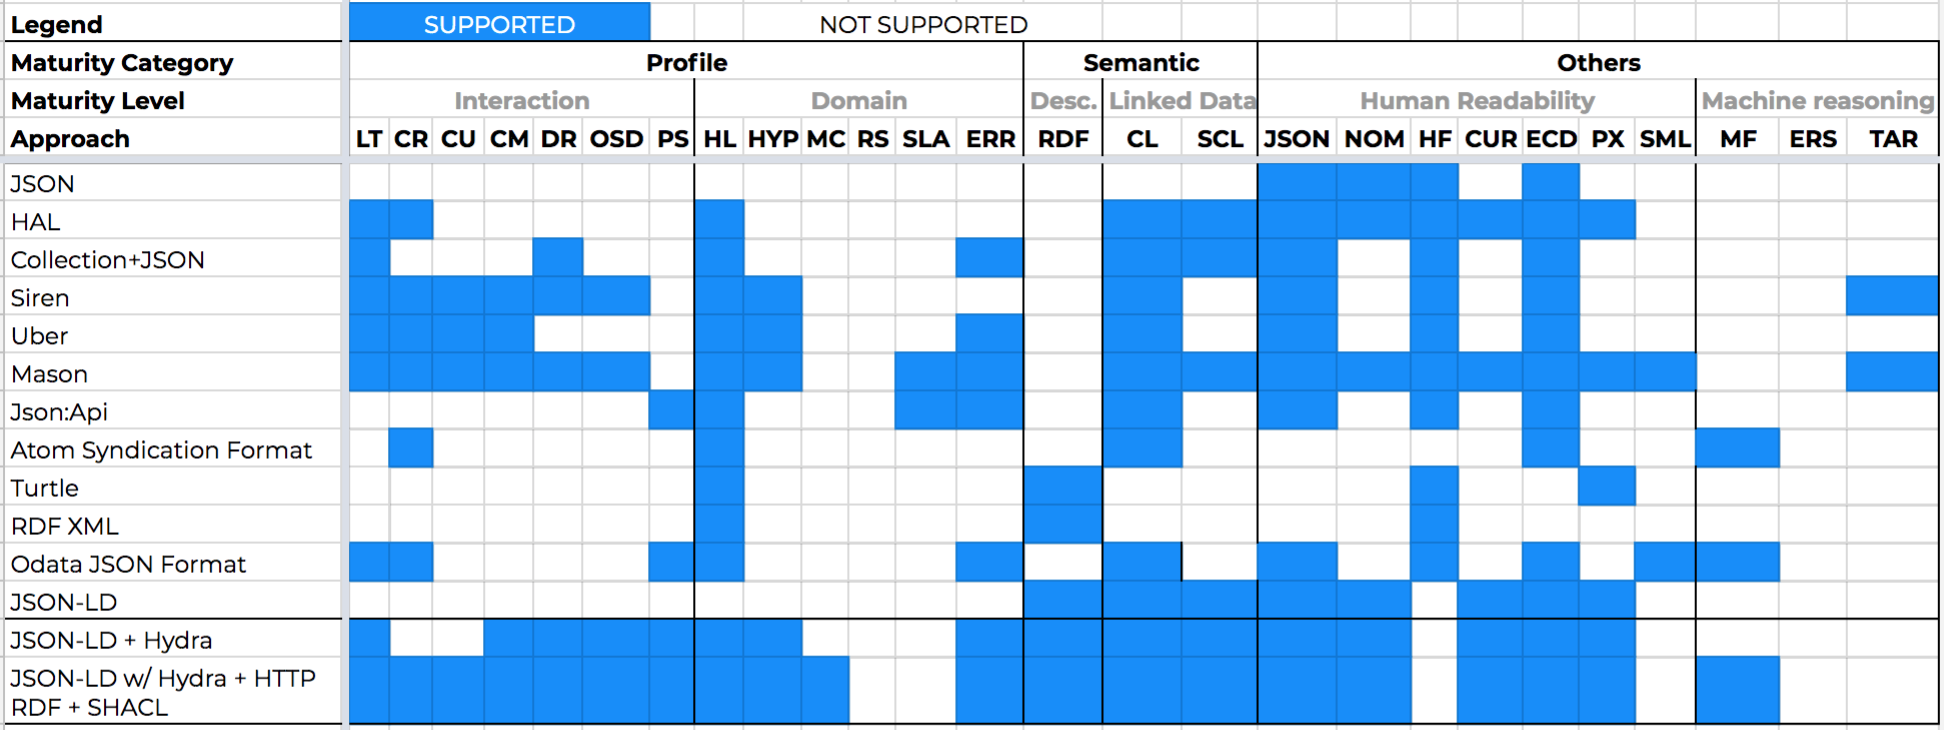
\includegraphics[width=1\textwidth]{figures/DIF.png}
\label{interchange-formats-matrix}
\end{figure*}

\subsubsection*{Conclusions}

On the one hand, non-RDF formats do not allow to reach any level on the semantic axis. However, some of them allow to link the data to others, and to reach the highest level on the \textit{Profile} dimension.
On the other hand, RDF formats can become very expressive when combined with vocabularies. The example with JSON-LD + Hydra + HTTP RDF + SCHACL shows this. However, they require more effort to find appropriate vocabularies on the web.
Furthermore, the matrix highlights that most formats are not readable by machine.

Last, the matrix shows that no format supports the description of constraints on the data neither the advertisement of resource's state. Though, most scientific approaches we found describe REST APIs as state machines. Providing the resource's state would ease machine-reasoning. On the other hand, describing the constraints could greatly decrease coupling and increase user experience. % TODO -> move to discussion

\subsection{Implementation Frameworks}

Implementation frameworks are software libraries that guide developers through the implementation of Web APIs. We limit the comparison to frameworks that claim to support HATEOAS. We identified six frameworks that do so.

In \cite{salvadori2014framework} authors propose \textit{Hypermedia Web API Support}, a Java framework based on JAX-RS 2.0 that uses annotations to semantically describe REST APIs. The end result is a JSON-LD document, enriched with the Hydra vocabulary, that describes the whole API. In \cite{parastatidis2010role} Parastatidis et al. present Restfulie, a framework to ease the development of REST APIs using resources, content-negotiation and state transitions as its core building blocks. Besides these frameworks, we found that API-Platform, Spring HATEOAS, JAX-RS and Ripozo support HATEOAS features. They are classified in Fig. \ref{frameworks-matrix} according to 29 criteria. % TODO: update the number of criteria

% FIGURE OF THE IMPLEMENTATION FRAMEWORKS CLASSIFICATION
\begin{figure*}[Ht]
\caption{Implementation Frameworks Comparison Matrix}
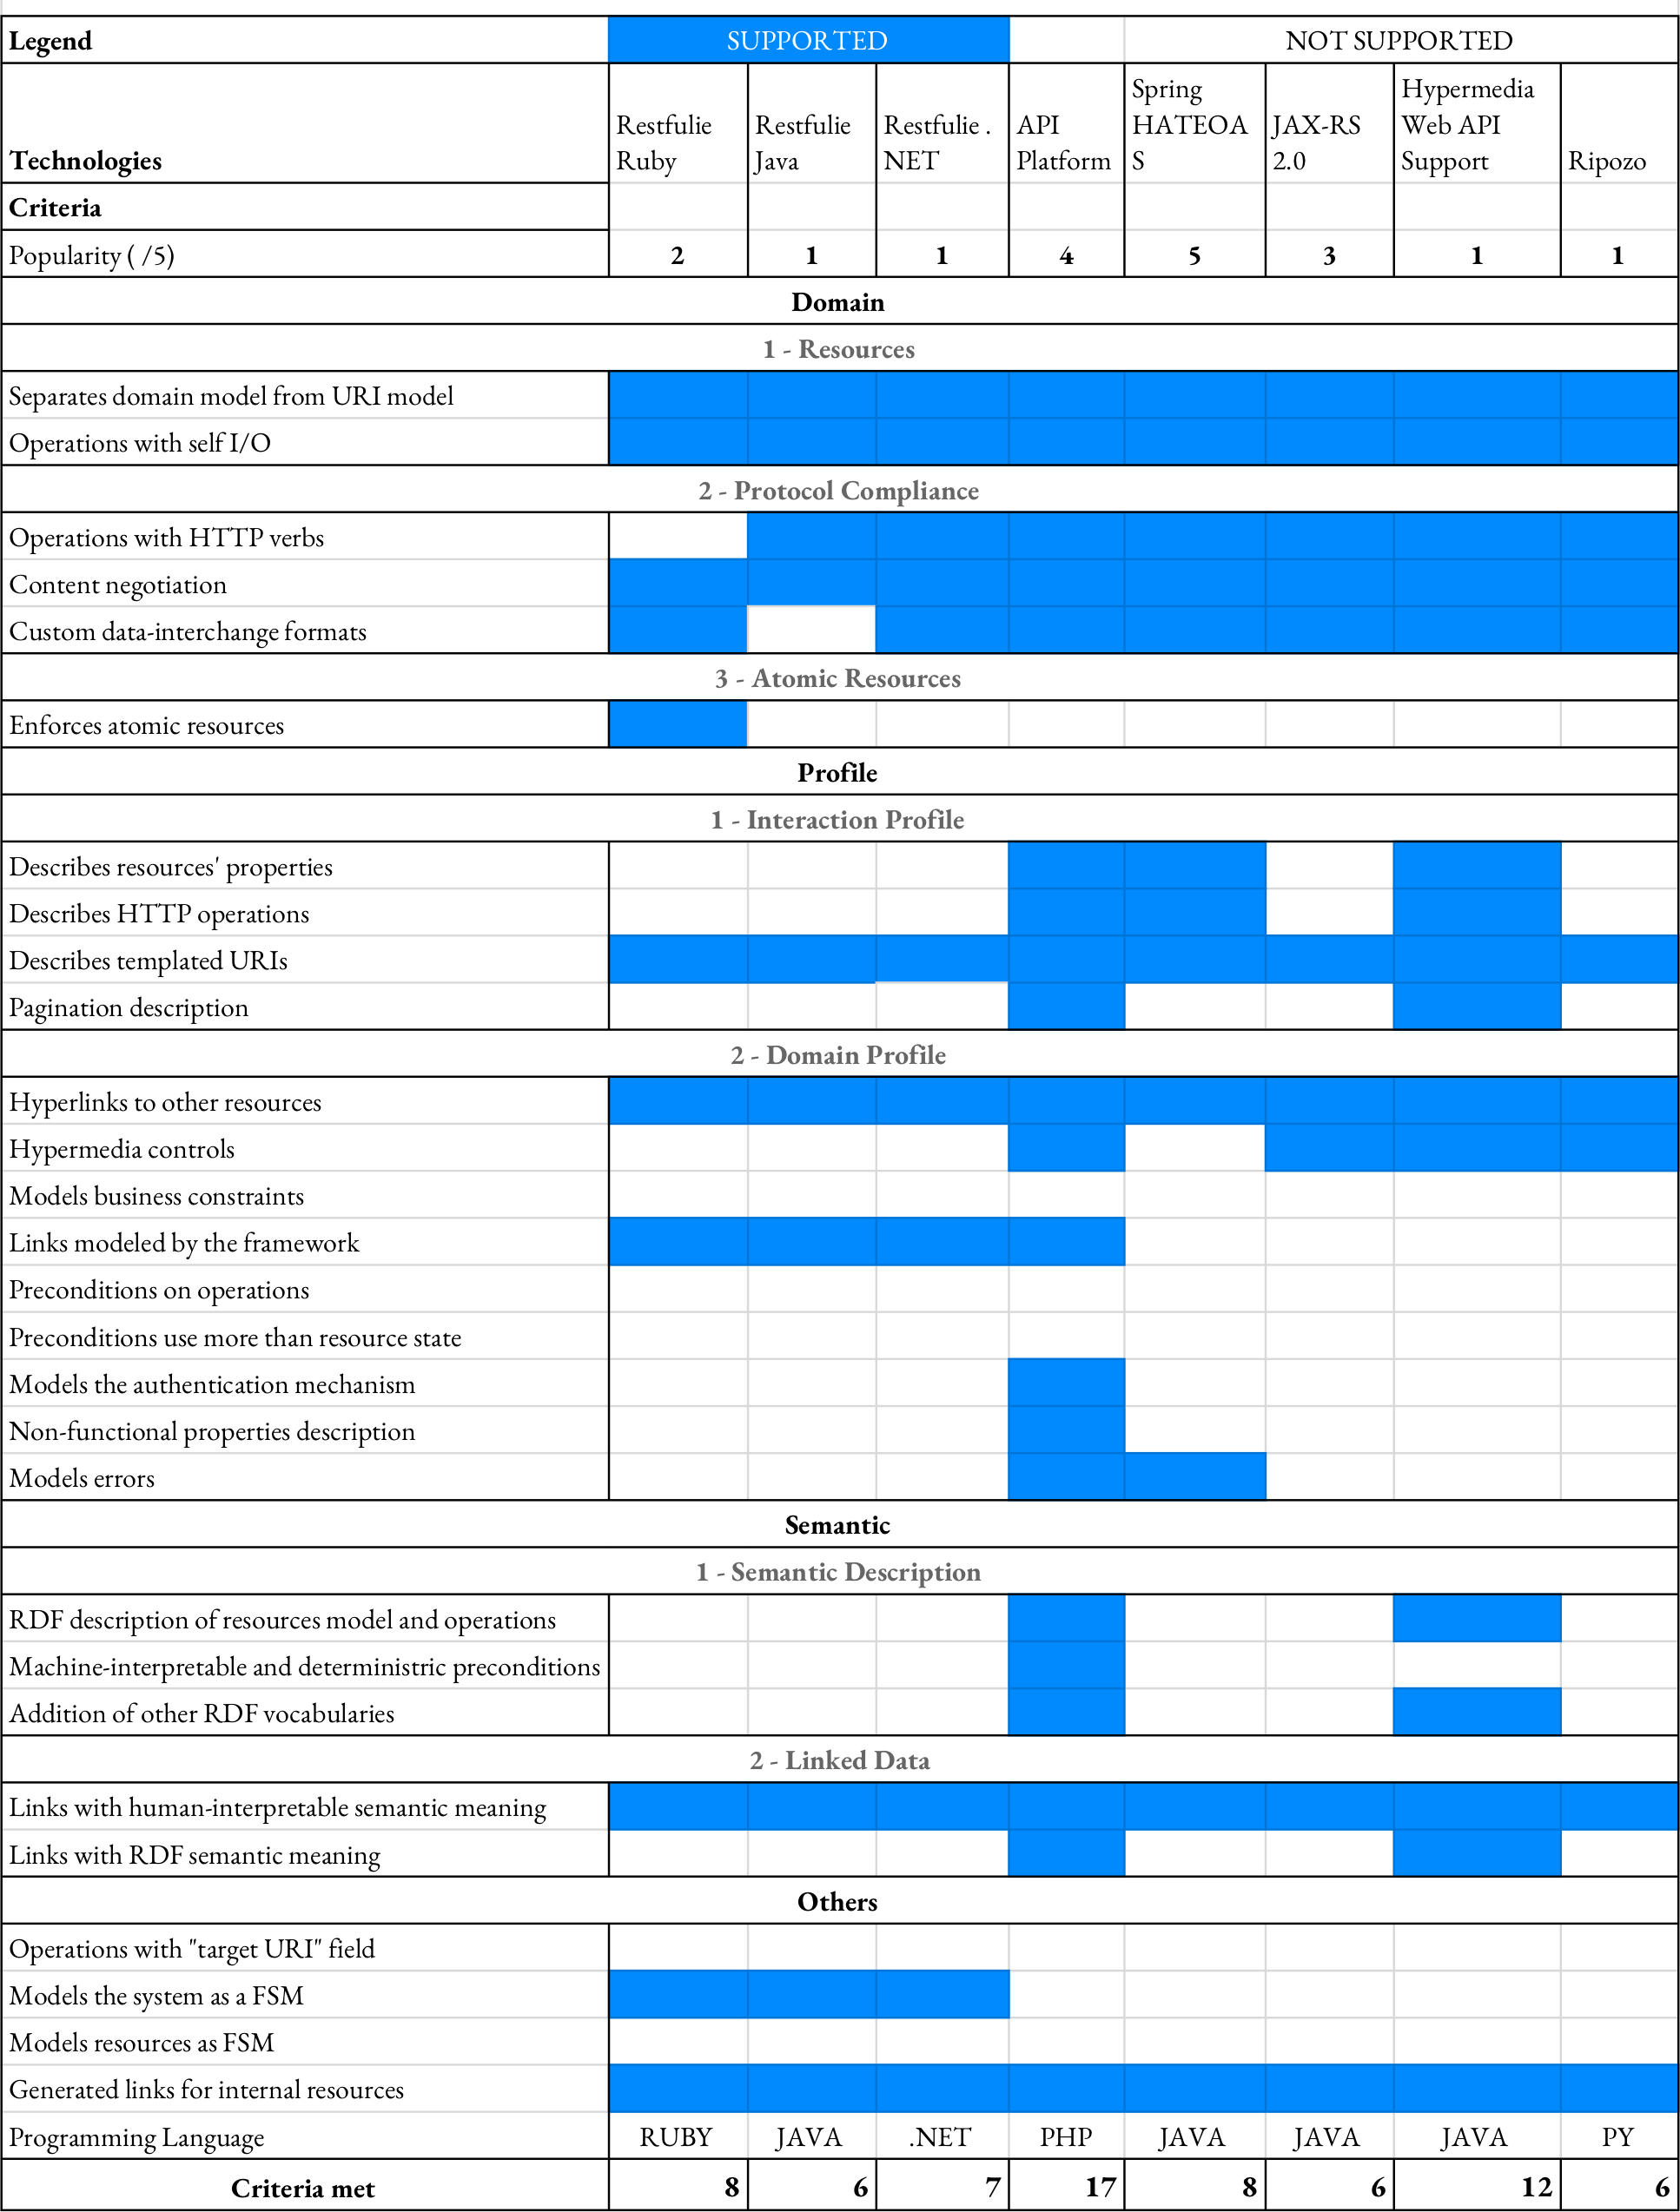
\includegraphics[width=1\textwidth]{figures/frameworks.png}
\label{frameworks-matrix}
\end{figure*}

\subsubsection*{Conclusions}

Despite the fact that only one framework enforces the atomic resources constraint, all frameworks allow to reach the highest level of maturity on the Design axis easily. This is because supporting the Atomic feature is a constraint that can be easily added by the developers themselves. 

We notice that only \textit{API Platform} and \textit{Restfulie} support a mechanism to model links instead of adding them programmatically in the resource or controller, thus increasing maintainability.

Otherwise, most framework do not ease the process of documenting and making the API Semantic Web and Linked Data compatible. To us, this is the biggest challenge framework designers are facing today.

As with IDLs, most creators of frameworks do not provide mechanisms to describe resources as state machines even though it could bring the same benefits. % TODO -> move to discussion
